\documentclass{standalone}
\usepackage{tikz}
\usetikzlibrary{patterns, positioning}


\begin{document}
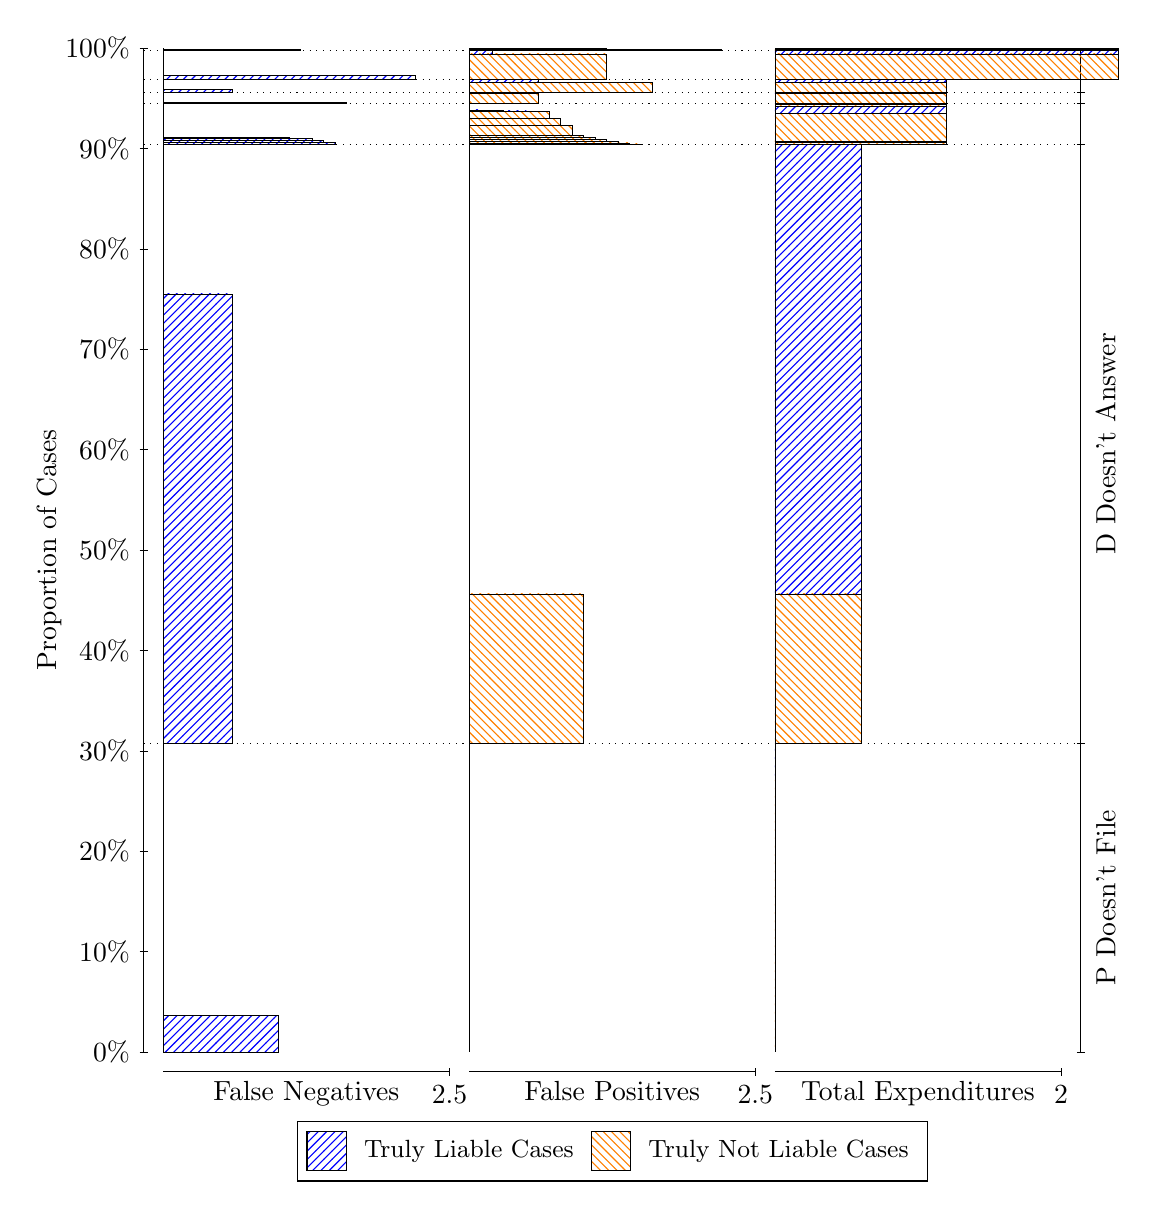
\begin{tikzpicture}
\draw[black, very thin] (1.5,1.75) -- (1.5,14.5);
\node[rotate=90, text=black, anchor=center] at (0.3, 8.125) {Proportion of Cases};
\draw[black, very thin] (1.45,1.75) -- (1.55,1.75);
\node[text=black, anchor=east] at (1.45, 1.75) {0\%};
\draw[black, very thin] (1.45,3.025) -- (1.55,3.025);
\node[text=black, anchor=east] at (1.45, 3.025) {10\%};
\draw[black, very thin] (1.45,4.3) -- (1.55,4.3);
\node[text=black, anchor=east] at (1.45, 4.3) {20\%};
\draw[black, very thin] (1.45,5.575) -- (1.55,5.575);
\node[text=black, anchor=east] at (1.45, 5.575) {30\%};
\draw[black, very thin] (1.45,6.85) -- (1.55,6.85);
\node[text=black, anchor=east] at (1.45, 6.85) {40\%};
\draw[black, very thin] (1.45,8.125) -- (1.55,8.125);
\node[text=black, anchor=east] at (1.45, 8.125) {50\%};
\draw[black, very thin] (1.45,9.4) -- (1.55,9.4);
\node[text=black, anchor=east] at (1.45, 9.4) {60\%};
\draw[black, very thin] (1.45,10.675) -- (1.55,10.675);
\node[text=black, anchor=east] at (1.45, 10.675) {70\%};
\draw[black, very thin] (1.45,11.95) -- (1.55,11.95);
\node[text=black, anchor=east] at (1.45, 11.95) {80\%};
\draw[black, very thin] (1.45,13.225) -- (1.55,13.225);
\node[text=black, anchor=east] at (1.45, 13.225) {90\%};
\draw[black, very thin] (1.45,14.5) -- (1.55,14.5);
\node[text=black, anchor=east] at (1.45, 14.5) {100\%};

\draw[black, very thin] (13.4,1.75) -- (13.4,14.5);
\draw[black, very thin] (13.35,1.75) -- (13.45,1.75);
\node[anchor=west] at (13.35, 1.75) {};
\draw[black, very thin] (13.35,5.6694) -- (13.45,5.6694);
\node[anchor=west] at (13.35, 5.6694) {};
\draw[black, very thin] (13.35,13.275) -- (13.45,13.275);
\node[anchor=west] at (13.35, 13.275) {};
\draw[black, very thin] (13.35,13.795) -- (13.45,13.795);
\node[anchor=west] at (13.35, 13.795) {};
\draw[black, very thin] (13.35,13.936) -- (13.45,13.936);
\node[anchor=west] at (13.35, 13.936) {};
\draw[black, very thin] (13.35,14.103) -- (13.45,14.103);
\node[anchor=west] at (13.35, 14.103) {};
\draw[black, very thin] (13.35,14.47) -- (13.45,14.47);
\node[anchor=west] at (13.35, 14.47) {};
\draw[black, very thin] (13.35,14.5) -- (13.45,14.5);
\node[anchor=west] at (13.35, 14.5) {};

\draw[black, very thin, pattern color=blue, pattern=north east lines] (1.75,1.75) rectangle (3.2033,2.2151);
\draw[black, very thin, pattern color=orange, pattern=north west lines] (1.75,2.2151) rectangle (1.75,5.6694);
\draw[black, very thin, pattern color=blue, pattern=north east lines] (1.75,5.6694) rectangle (2.622,11.377);
\draw[black, very thin, pattern color=orange, pattern=north west lines] (1.75,11.377) rectangle (1.75,13.275);
\draw[black, very thin, pattern color=blue, pattern=north east lines] (1.75,13.275) rectangle (3.93,13.301);
\draw[black, very thin, pattern color=blue, pattern=north east lines] (1.75,13.301) rectangle (3.7847,13.323);
\draw[black, very thin, pattern color=blue, pattern=north east lines] (1.75,13.323) rectangle (3.6393,13.35);
\draw[black, very thin, pattern color=blue, pattern=north east lines] (1.75,13.35) rectangle (3.494,13.355);
\draw[black, very thin, pattern color=blue, pattern=north east lines] (1.75,13.355) rectangle (3.3487,13.361);
\draw[black, very thin, pattern color=blue, pattern=north east lines] (1.75,13.361) rectangle (3.2033,13.365);
\draw[black, very thin, pattern color=blue, pattern=north east lines] (1.75,13.365) rectangle (3.058,13.367);
\draw[black, very thin, pattern color=blue, pattern=north east lines] (1.75,13.367) rectangle (2.9127,13.369);
\draw[black, very thin, pattern color=blue, pattern=north east lines] (1.75,13.369) rectangle (2.7673,13.37);
\draw[black, very thin, pattern color=orange, pattern=north west lines] (1.75,13.37) rectangle (1.75,13.795);
\draw[black, very thin, pattern color=blue, pattern=north east lines] (1.75,13.795) rectangle (4.0753,13.806);
\draw[black, very thin, pattern color=orange, pattern=north west lines] (1.75,13.806) rectangle (1.75,13.936);
\draw[black, very thin, pattern color=blue, pattern=north east lines] (1.75,13.936) rectangle (2.622,13.973);
\draw[black, very thin, pattern color=orange, pattern=north west lines] (1.75,13.973) rectangle (1.75,14.103);
\draw[black, very thin, pattern color=blue, pattern=north east lines] (1.75,14.103) rectangle (4.9473,14.148);
\draw[black, very thin, pattern color=orange, pattern=north west lines] (1.75,14.148) rectangle (1.75,14.47);
\draw[black, very thin, pattern color=blue, pattern=north east lines] (1.75,14.47) rectangle (3.494,14.484);
\draw[black, very thin, pattern color=orange, pattern=north west lines] (1.75,14.484) rectangle (1.75,14.5);
\draw[black, very thin, pattern color=orange, pattern=north west lines] (5.6333,1.75) rectangle (5.6333,5.2043);
\draw[black, very thin, pattern color=blue, pattern=north east lines] (5.6333,5.2043) rectangle (5.6333,5.6694);
\draw[black, very thin, pattern color=orange, pattern=north west lines] (5.6333,5.6694) rectangle (7.0867,7.5677);
\draw[black, very thin, pattern color=blue, pattern=north east lines] (5.6333,7.5677) rectangle (5.6333,13.275);
\draw[black, very thin, pattern color=orange, pattern=north west lines] (5.6333,13.275) rectangle (7.8133,13.282);
\draw[black, very thin, pattern color=orange, pattern=north west lines] (5.6333,13.282) rectangle (7.668,13.294);
\draw[black, very thin, pattern color=orange, pattern=north west lines] (5.6333,13.294) rectangle (7.5227,13.314);
\draw[black, very thin, pattern color=orange, pattern=north west lines] (5.6333,13.314) rectangle (7.3773,13.336);
\draw[black, very thin, pattern color=orange, pattern=north west lines] (5.6333,13.336) rectangle (7.232,13.368);
\draw[black, very thin, pattern color=orange, pattern=north west lines] (5.6333,13.368) rectangle (7.0867,13.393);
\draw[black, very thin, pattern color=orange, pattern=north west lines] (5.6333,13.393) rectangle (6.9413,13.516);
\draw[black, very thin, pattern color=orange, pattern=north west lines] (5.6333,13.516) rectangle (6.796,13.602);
\draw[black, very thin, pattern color=orange, pattern=north west lines] (5.6333,13.602) rectangle (6.6507,13.7);
\draw[black, very thin, pattern color=blue, pattern=north east lines] (5.6333,13.7) rectangle (6.36,13.701);
\draw[black, very thin, pattern color=blue, pattern=north east lines] (5.6333,13.701) rectangle (6.2147,13.703);
\draw[black, very thin, pattern color=blue, pattern=north east lines] (5.6333,13.703) rectangle (6.0693,13.705);
\draw[black, very thin, pattern color=blue, pattern=north east lines] (5.6333,13.705) rectangle (5.924,13.709);
\draw[black, very thin, pattern color=blue, pattern=north east lines] (5.6333,13.709) rectangle (5.7787,13.715);
\draw[black, very thin, pattern color=blue, pattern=north east lines] (5.6333,13.715) rectangle (5.6333,13.795);
\draw[black, very thin, pattern color=orange, pattern=north west lines] (5.6333,13.795) rectangle (6.5053,13.925);
\draw[black, very thin, pattern color=blue, pattern=north east lines] (5.6333,13.925) rectangle (5.6333,13.936);
\draw[black, very thin, pattern color=orange, pattern=north west lines] (5.6333,13.936) rectangle (7.9587,14.066);
\draw[black, very thin, pattern color=blue, pattern=north east lines] (5.6333,14.066) rectangle (6.5053,14.103);
\draw[black, very thin, pattern color=orange, pattern=north west lines] (5.6333,14.103) rectangle (7.3773,14.426);
\draw[black, very thin, pattern color=blue, pattern=north east lines] (5.6333,14.426) rectangle (5.924,14.47);
\draw[black, very thin, pattern color=orange, pattern=north west lines] (5.6333,14.47) rectangle (8.8307,14.486);
\draw[black, very thin, pattern color=blue, pattern=north east lines] (5.6333,14.486) rectangle (7.3773,14.5);
\draw[black, very thin, pattern color=orange, pattern=north west lines] (9.5167,1.75) rectangle (9.5167,5.2043);
\draw[black, very thin, pattern color=blue, pattern=north east lines] (9.5167,5.2043) rectangle (9.5167,5.6694);
\draw[black, very thin, pattern color=orange, pattern=north west lines] (9.5167,5.6694) rectangle (10.607,7.5677);
\draw[black, very thin, pattern color=blue, pattern=north east lines] (9.5167,7.5677) rectangle (10.607,13.275);
\draw[black, very thin, pattern color=orange, pattern=north west lines] (9.5167,13.275) rectangle (11.697,13.308);
\draw[black, very thin, pattern color=blue, pattern=north east lines] (9.5167,13.308) rectangle (11.697,13.314);
\draw[black, very thin, pattern color=orange, pattern=north west lines] (9.5167,13.314) rectangle (11.697,13.674);
\draw[black, very thin, pattern color=blue, pattern=north east lines] (9.5167,13.674) rectangle (11.697,13.758);
\draw[black, very thin, pattern color=orange, pattern=north west lines] (9.5167,13.758) rectangle (11.697,13.79);
\draw[black, very thin, pattern color=blue, pattern=north east lines] (9.5167,13.79) rectangle (11.697,13.795);
\draw[black, very thin, pattern color=orange, pattern=north west lines] (9.5167,13.795) rectangle (11.697,13.925);
\draw[black, very thin, pattern color=blue, pattern=north east lines] (9.5167,13.925) rectangle (11.697,13.936);
\draw[black, very thin, pattern color=orange, pattern=north west lines] (9.5167,13.936) rectangle (11.697,14.066);
\draw[black, very thin, pattern color=blue, pattern=north east lines] (9.5167,14.066) rectangle (11.697,14.103);
\draw[black, very thin, pattern color=orange, pattern=north west lines] (9.5167,14.103) rectangle (13.877,14.426);
\draw[black, very thin, pattern color=blue, pattern=north east lines] (9.5167,14.426) rectangle (13.877,14.47);
\draw[black, very thin, pattern color=orange, pattern=north west lines] (9.5167,14.47) rectangle (13.877,14.486);
\draw[black, very thin, pattern color=blue, pattern=north east lines] (9.5167,14.486) rectangle (13.877,14.5);
\draw[black, dotted] (1.5,5.6694) -- (13.4,5.6694);
\draw[black, dotted] (1.5,13.275) -- (13.4,13.275);
\draw[black, dotted] (1.5,13.795) -- (13.4,13.795);
\draw[black, dotted] (1.5,13.936) -- (13.4,13.936);
\draw[black, dotted] (1.5,14.103) -- (13.4,14.103);
\draw[black, dotted] (1.5,14.47) -- (13.4,14.47);
\draw[black, very thin] (1.75,1.5) -- (5.3833,1.5);
\node[text=black, anchor=north] at (3.5667, 1.5) {False Negatives};
\draw[black, very thin] (5.3833,1.45) -- (5.3833,1.55);
\node[text=black, anchor=north] at (5.3833, 1.45) {2.5};

\draw[black, very thin] (5.6333,1.5) -- (9.2667,1.5);
\node[text=black, anchor=north] at (7.45, 1.5) {False Positives};
\draw[black, very thin] (9.2667,1.45) -- (9.2667,1.55);
\node[text=black, anchor=north] at (9.2667, 1.45) {2.5};

\draw[black, very thin] (9.5167,1.5) -- (13.15,1.5);
\node[text=black, anchor=north] at (11.333, 1.5) {Total Expenditures};
\draw[black, very thin] (13.15,1.45) -- (13.15,1.55);
\node[text=black, anchor=north] at (13.15, 1.45) {2};

\node[text=black, centered, rotate=90] at (13.72, 3.7097) {P Doesn't File};
\node[text=black, centered, rotate=90] at (13.72, 9.4723) {D Doesn't Answer};






\draw (7.449999999999999,1.5) node[draw=none] (baseCoordinate) {};
\begin{scope}[align=center]
        \matrix[scale=0.5, draw=black, below=0.5cm of baseCoordinate, nodes={draw}, column sep=0.1cm]{
            \node[rectangle, draw, minimum width=0.5cm, minimum height=0.5cm, pattern color=blue, pattern=north east lines] {}; &
            \node[draw=none, font=\small, text=black] (B) {Truly Liable Cases}; &
            \node[rectangle, draw, minimum width=0.5cm, minimum height=0.5cm, pattern color=orange, pattern=north west lines] {}; &
            \node[draw=none, font=\small, text=black] (B) {Truly Not Liable Cases}; \\
            };
\end{scope}

\end{tikzpicture}
\end{document}